\documentclass[a4paper, 14pt]{extarticle}

% Поля
%--------------------------------------
\usepackage{geometry}
\geometry{a4paper,tmargin=2cm,bmargin=2cm,lmargin=3cm,rmargin=1cm}
%--------------------------------------


%Russian-specific packages
%--------------------------------------
\usepackage[T2A]{fontenc}
\usepackage[utf8]{inputenc} 
\usepackage[english, main=russian]{babel}
%--------------------------------------

\usepackage{textcomp}

% Красная строка
%--------------------------------------
\usepackage{indentfirst}               
%--------------------------------------             


%Graphics
%--------------------------------------
\usepackage{graphicx}
\graphicspath{ {./images/} }
\usepackage{wrapfig}
%--------------------------------------

% Полуторный интервал
%--------------------------------------
\linespread{1.3}                    
%--------------------------------------

%Выравнивание и переносы
%--------------------------------------
% Избавляемся от переполнений
\sloppy
% Запрещаем разрыв страницы после первой строки абзаца
\clubpenalty=10000
% Запрещаем разрыв страницы после последней строки абзаца
\widowpenalty=10000
%--------------------------------------

%Списки
\usepackage{enumitem}

%Подписи
\usepackage{caption} 

%Гиперссылки
\usepackage{hyperref}

\hypersetup {
	unicode=true
}

%Рисунки
%--------------------------------------
\DeclareCaptionLabelSeparator*{emdash}{~--- }
\captionsetup[figure]{labelsep=emdash,font=onehalfspacing,position=bottom}
%--------------------------------------

\usepackage{tempora}

%Листинги
%--------------------------------------
\usepackage{listings}
\lstset{
  basicstyle=\ttfamily\footnotesize, 
  %basicstyle=\footnotesize\AnkaCoder,        % the size of the fonts that are used for the code
  breakatwhitespace=false,         % sets if automatic breaks shoulbd only happen at whitespace
  breaklines=true,                 % sets automatic line breaking
  captionpos=t,                    % sets the caption-position to bottom
  inputencoding=utf8,
  frame=single,                    % adds a frame around the code
  keepspaces=true,                 % keeps spaces in text, useful for keeping indentation of code (possibly needs columns=flexible)
  keywordstyle=\bf,       % keyword style
  numbers=left,                    % where to put the line-numbers; possible values are (none, left, right)
  numbersep=5pt,                   % how far the line-numbers are from the code
  xleftmargin=25pt,
  xrightmargin=25pt,
  showspaces=false,                % show spaces everywhere adding particular underscores; it overrides 'showstringspaces'
  showstringspaces=false,          % underline spaces within strings only
  showtabs=false,                  % show tabs within strings adding particular underscores
  stepnumber=1,                    % the step between two line-numbers. If it's 1, each line will be numbered
  tabsize=2,                       % sets default tabsize to 8 spaces
  title=\lstname                   % show the filename of files included with \lstinputlisting; also try caption instead of title
}
%--------------------------------------

%%% Математические пакеты %%%
%--------------------------------------
\usepackage{amsthm,amsfonts,amsmath,amssymb,amscd}  % Математические дополнения от AMS
\usepackage{mathtools}                              % Добавляет окружение multlined
\usepackage[perpage]{footmisc}
%--------------------------------------

%--------------------------------------
%			НАЧАЛО ДОКУМЕНТА
%--------------------------------------

\begin{document}

%--------------------------------------
%			ТИТУЛЬНЫЙ ЛИСТ
%--------------------------------------
\begin{titlepage}
\thispagestyle{empty}
\newpage


%Шапка титульного листа
%--------------------------------------
\vspace*{-60pt}
\hspace{-65pt}
\begin{minipage}{0.3\textwidth}
\hspace*{-20pt}\centering

\includegraphics[width=\textwidth]{emblem}
\end{minipage}
\begin{minipage}{0.67\textwidth}\small \textbf{
\vspace*{-0.7ex}
\hspace*{-6pt}\centerline{Министерство науки и высшего образования Российской Федерации}
\vspace*{-0.7ex}
\centerline{Федеральное государственное бюджетное образовательное учреждение }
\vspace*{-0.7ex}
\centerline{высшего образования}
\vspace*{-0.7ex}
\centerline{<<Московский государственный технический университет}
\vspace*{-0.7ex}
\centerline{имени Н.Э. Баумана}
\vspace*{-0.7ex}
\centerline{(национальный исследовательский университет)>>}
\vspace*{-0.7ex}
\centerline{(МГТУ им. Н.Э. Баумана)}}
\end{minipage}
%--------------------------------------

%Полосы
%--------------------------------------
\vspace{-25pt}
\hspace{-35pt}\rule{\textwidth}{2.3pt}

\vspace*{-20.3pt}
\hspace{-35pt}\rule{\textwidth}{0.4pt}
%--------------------------------------

\vspace{1.5ex}
\hspace{-35pt} \noindent \small ФАКУЛЬТЕТ\hspace{80pt} <<Информатика и системы управления>>

\vspace*{-16pt}
\hspace{47pt}\rule{0.83\textwidth}{0.4pt}

\vspace{0.5ex}
\hspace{-35pt} \noindent \small КАФЕДРА\hspace{50pt} <<Теоретическая информатика и компьютерные технологии>>

\vspace*{-16pt}
\hspace{30pt}\rule{0.866\textwidth}{0.4pt}
  
\vspace{11em}

\begin{center}
\Large {\bf Лабораторная работа № 3} \\ 
\large {\bf по курсу <<Языки и методы программирования>>} \\
\large <<Полиморфизм на основе интерфейсов в языке Java>> 
\end{center}\normalsize

\vspace{8em}


\begin{flushright}
  {Студент группы ИУ9-21Б Горбунов А. Д. \hspace*{15pt}\\ 
  \vspace{2ex}
  Преподаватель Посевин Д. П.\hspace*{15pt}}
\end{flushright}

\bigskip

\vfill
 

\begin{center}
\textsl{Москва 2023}
\end{center}
\end{titlepage}
%--------------------------------------
%		КОНЕЦ ТИТУЛЬНОГО ЛИСТА
%--------------------------------------

\renewcommand{\ttdefault}{pcr}

\setlength{\tabcolsep}{3pt}
\newpage
\setcounter{page}{2}

\section{Задание}\label{Sect::task}
Во время выполнения лабораторной работы требуется разработать на языке Java один из 
классов, перечисленных в таблице. В классе должен быть реализован интерфейс Comparable<T> и переопределён метод toString. В методе main вспомогательного класса Test нужно продемонстрировать работоспособность разработанного класса путём сортировки массива его экземпляров.

Класс полиномов с порядком на основе количества целочисленных корней, принадлежащих интервалу [0; 10].
\section{Результаты}\label{Sect::res}

Исходный код программы представлен в листинге~\ref{lst:code1}, ~\ref{lst:code2}.

\begin{figure}[!htb]
\begin{lstlisting}[language={},caption={класс Test},label={lst:code1}]
import java.util.Arrays;
public class Test {
    public static void main(String[] args) {
        Polynomial[] polynomials = new Polynomial[5];
        polynomials[0] = new Polynomial(new int[]{1, 0, -1});
        polynomials[1] = new Polynomial(new int[]{1, 0, 0, -1});
        polynomials[2] = new Polynomial(new int[]{1, 0, 1, 0, -1});
        polynomials[3] = new Polynomial(new int[]{1, 1, 1});
        polynomials[4] = new Polynomial(new int[]{1, -1});
        Arrays.sort(polynomials);
        for (Polynomial p : polynomials) {
            System.out.println(p);
        }
    }
}
\end{lstlisting}
\end{figure}

\begin{figure}[!htb]
\begin{lstlisting}[language={},caption={класс Polynomial},label={lst:code2}]
public class Polynomial implements Comparable<Polynomial> {
    private int[] a_n;
    public Polynomial(int[] a_n) {
        this.a_n = a_n;
    }
    public int getNumberOfIntegerRoots() {
        int count = 0;
        for (int i = 0; i <= 10; i++)
            if (evaluate(i) < 0.001)
                count++;
        return count;
    }
    public double evaluate(int x) {
        double result = 0;
        for (int i = 0; i < a_n.length; i++)
            result += a_n[i] * Math.pow(x, i);
        return result;
    }
    @Override
    public int compareTo(Polynomial other) {
        return Integer.compare(this.getNumberOfIntegerRoots(), other.getNumberOfIntegerRoots());
    }
    @Override
    public String toString() {
        String result = "";
        for (int i = a_n.length - 1; i >= 0; i--)
            if (i == 0)
                result += (a_n[i] > 0 && i < a_n.length-1? "+" : "") + a_n[i];
            else if (a_n[i] != 0)
                result += (a_n[i] > 0 && i < a_n.length-1? "+" : "") + a_n[i] + "*x^" + i;
        return result;
    }



}
\end{lstlisting}
\end{figure}

\begin{figure}[!htb]
Результат запуска представлен на рисунке ~\ref{fig:picture_1.png}, ~\ref{fig:picture_2.png}.
\end{figure}

\begin{figure}[!htb]
	\centering
	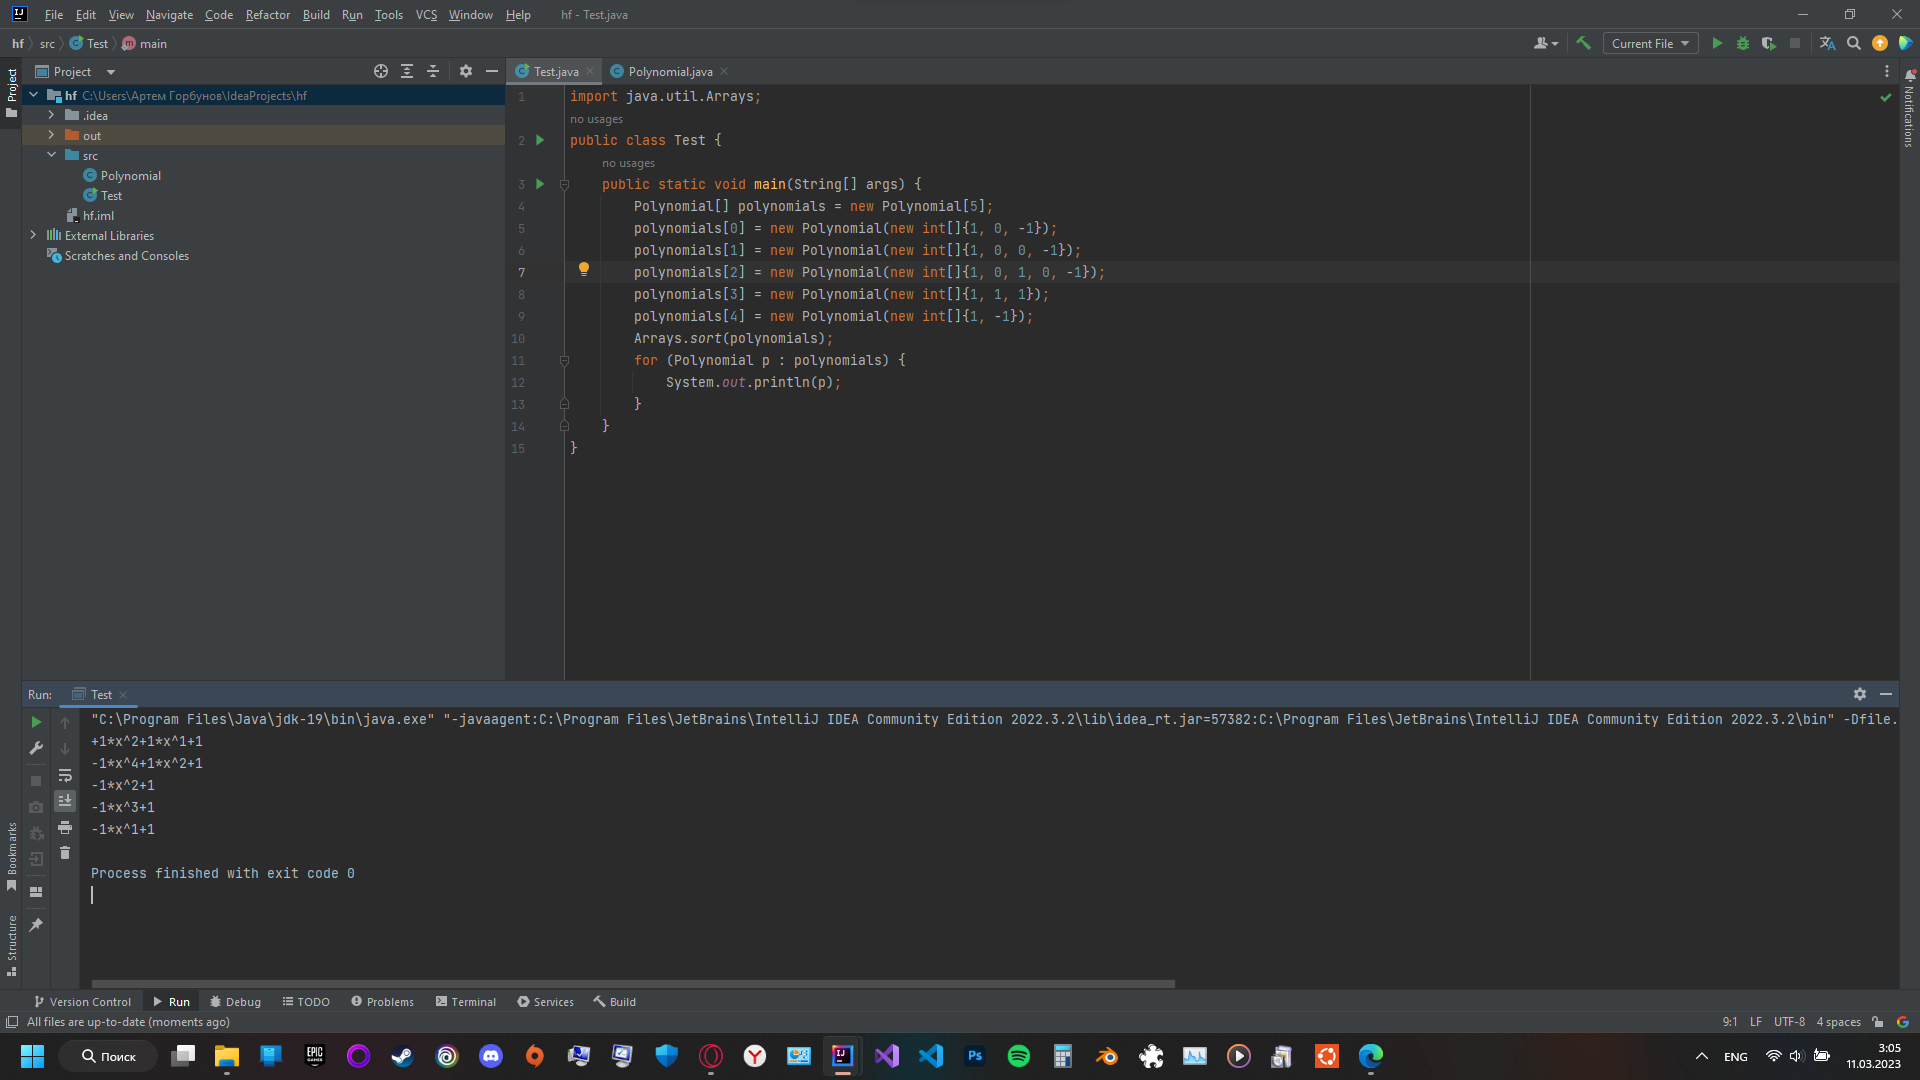
\includegraphics[width=0.8\textwidth]{picture_1.png}
\caption{Вывод программы}
\label{fig:picture_1.png}
\end{figure}

\begin{figure}[!htb]
	\centering
	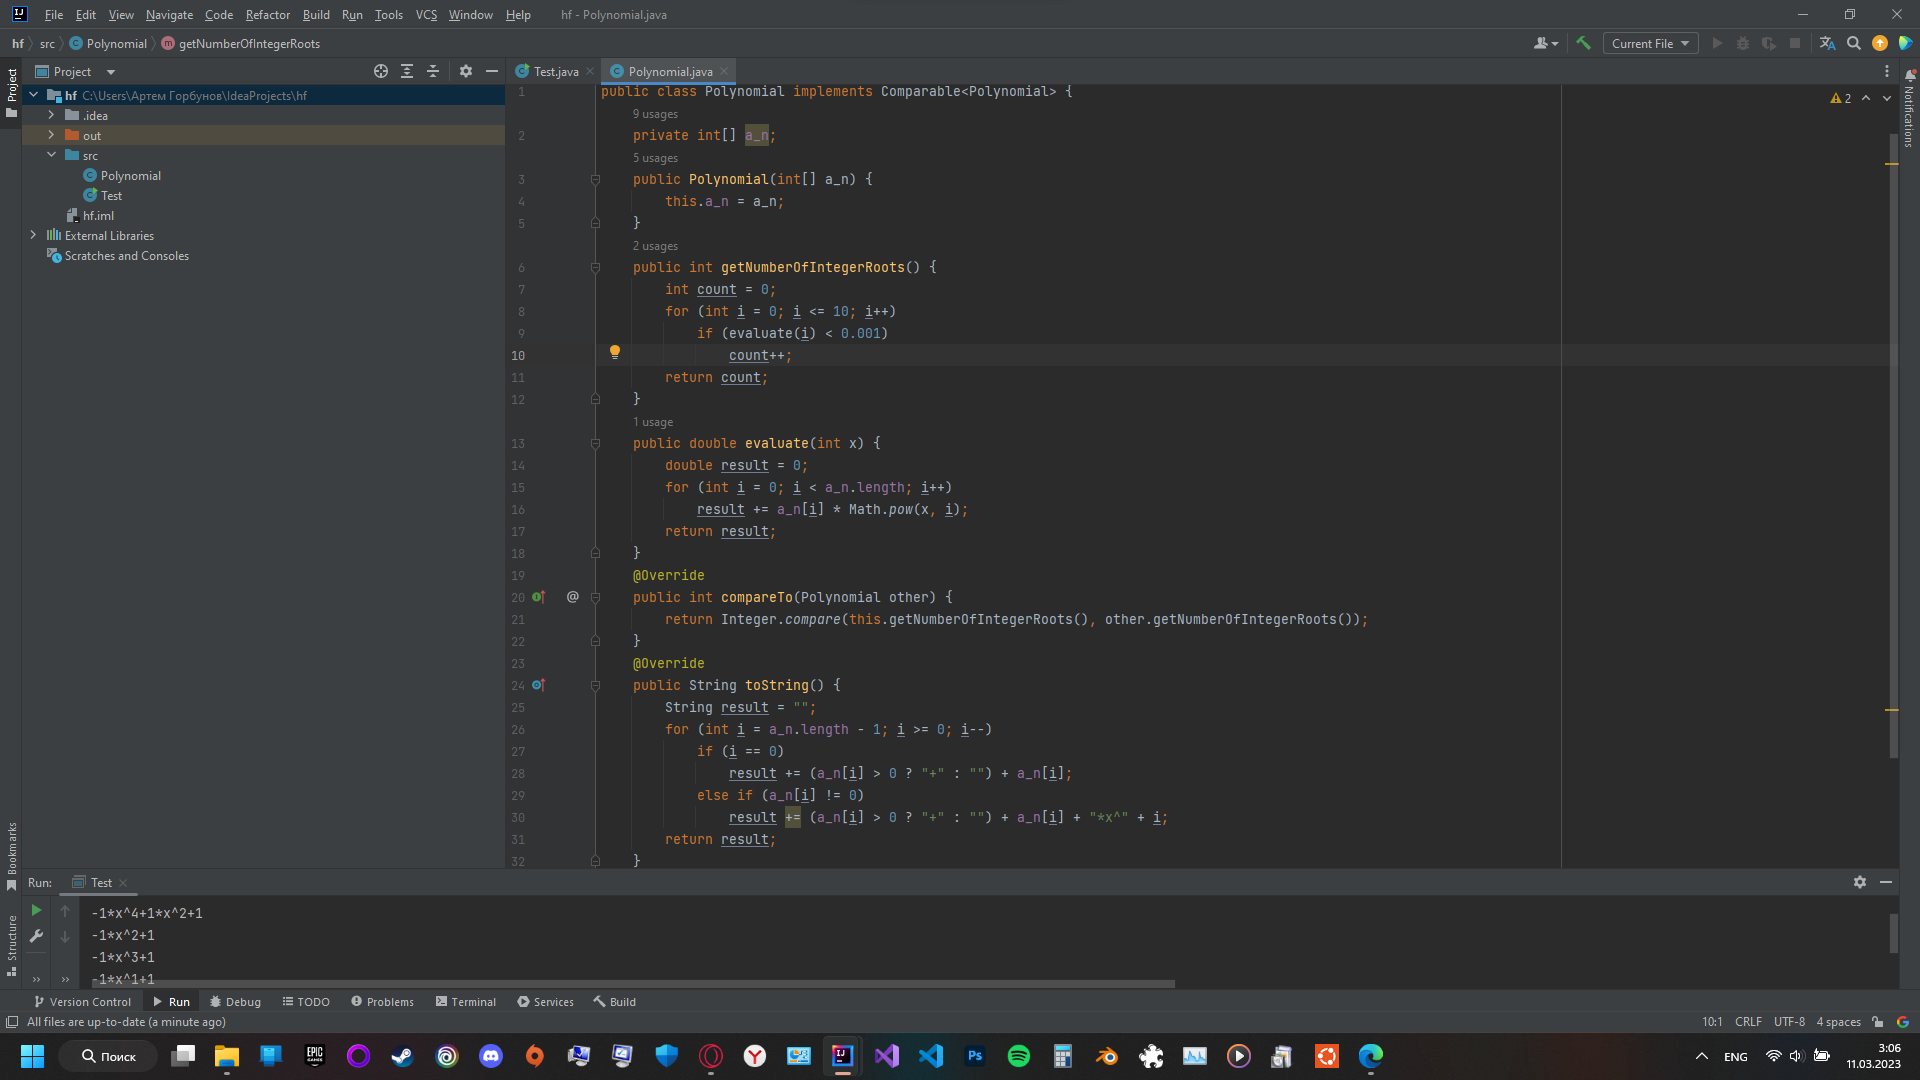
\includegraphics[width=0.8\textwidth]{picture_2.png}
\caption{Работа программы}
\label{fig:picture_2.png}
\end{figure}

\end{document}
